\documentclass[thesis.tex]{subfiles}
\begin{document}

\chapter{Simulation}\label{chap:simulation}
%
\begin{figure}[ht!]
\centering
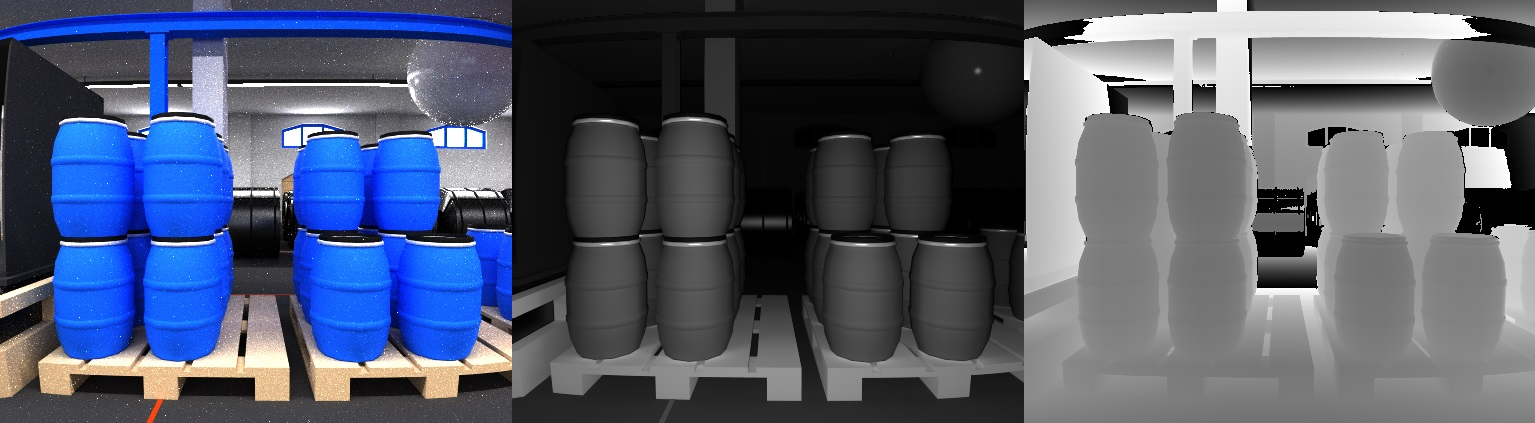
\includegraphics[width=1.0\linewidth]{simluation/sumulation_headline.jpg}
\caption{Screenshots der Simulation mit einem Farbbild, einem Infrarotbild und einem Tiefenbild.}
\label{fig:simulation_headline_image}
\end{figure}
Dieses Kapitel beschäftigt sich mit der Erläuterung der Time-of-Flight Sensor Simulation mittels Path Tracing und der Generierung der Tiefenbilder. Die Simulation lässt sich grob in zwei Phasen unterteilen. Zunächst wird die Simulation des Time-of-Flight Sensors und der Lichtausbreitung auf der GPU mittels Path Tracing durchgeführt. Das Ergebnis der Simulation sind die einzelnen Phasenbilder, die in \autoref{chap:time_of_flight} erläutert wurden. Mit Hilfe dieser Phasenbilder werden anschließend auf der CPU die Tiefenwerte unter Berücksichtigung des Lens Scattering und des zufälligen Fehlers berechnet.

In den folgenden Unterkapiteln werden daher zunächst der Path Tracing Algorithmus im Detail erläutert und im Anschluss die Berechnung der Tiefenwerte behandelt.
%
\section{Path Tracing}

\begin{figure}[ht!]
    \centering
    \includepdftex{path_tracing_concept}
    \caption{Schematische Darstellung der des Path Tracing Algorithmus mit zwei Pfaden für den selben Pixel.}
    \label{fig:path_tracing_concept}
\end{figure}

Bei dem Path Tacing Algorithmus handelt es sich um eine Implementierung nach Kajiya \cite{bib:Kajiya1986}. Dabei werden für jeden Pixel des Bildes Strahlen in die Szene geschickt. Anschließend wird bestimmt, ob der Strahl mit der Szene kollidiert. Falls dieser Strahl mit einer Oberfläche kollidiert, wird ermittelt, ob dieser Punkt von Lichtquellen beleuchtet wird und die anteilige Strahlung bestimmt, die in die Richtung des Betrachters reflektiert wird. Für die indirekte Beleuchtung durch andere Oberflächen wird ein neuer Strahl in eine zufällige Richtung bestimmt, der seinen Ursprung im Schnittpunkt hat. Es wird nun wiederholt ermittelt, ob dieser neue Strahl mit der Szene kollidiert und die Reflexion in Richtung des Ursprungs berechnet. Dies wird solange wiederholt, bis eine maximale Länge für den Pfad erreicht wurde, oder der Strahl die Szene verlässt. \autoref{fig:path_tracing_concept} veranschaulicht die Funktionsweise des Algorithmus für mehrere Sichtstrahlen, die für denselben Pixel berechnet werden. Dabei verlässt jeder Strahl den Betrachter in dieselbe Richtung und erhält für jeden Schnittpunkt jeweils eine zufällige neue Richtung. Für jeden Schnittpunkt wird dabei berechnet, ob dieser direkt durch eine oder mehrere Lichtquellen beleuchtet wird.

Der Path Tracing Algorithmus wurde unter Verwendung der NVIDIA OptiX Ray Tracing Engine entwickelt. Dabei handelt es sich um ein Framework, das eine API zur Erstellung von Ray Tracing Applikationen anbietet \cite{bib:Parker2010}. Daher wird neben der Installation von OptiX auch die des CUDA Toolkits benötigt und zur Verwendung dessen ist eine Grafikkarte notwendig, die CUDA unterstützt. Bei CUDA handelt es sich um eine API, die von NVIDIA entwickelt wurde und es dem Nutzer ermöglicht die Ausführung von Programmteilen mittels \emph{General-Purpose Computing on Graphics Processing Units} (GPGPU) auf der Grafikkarte durchführen zu lassen. Dabei zeichnet sich die Berechnung auf der Grafikkarte durch die hochgradig parallele Abarbeitung aus. Im Falle des Path Tracings kann für die Berechnung von jedem Strahl ein eigener Thread genutzt werden und so kann die Programmausführung für tausende von Strahlen gleichzeitig durchgeführt werden.

Das OptiX Framework bietet Schnittstellen an, in denen Teile der Funktionalität mittels CUDA C Kernels definiert werden können, die im Folgenden erläutert werden. Die Implementierung eines Path Tracing Algorithmus mittels OptiX involviert dabei folgende Schritte:
%
\begin{enumerate}
    \item die Implementierung eines \emph{Ray Generation} Programms, das definiert, wie die Strahlen in die Szene geschossen werden
    \item die Definition eines \emph{Bounding Box} Programms, welches zur Beschleunigung des Algorithmus benötigt wird und einen groben Test beschreibt und Feedback darüber gibt, ob der Strahl sich in der Nähe des Objektes befindet, bevor eine genaue und rechenintensive Schnittberechnung mit der Oberfläche des Objektes durchgeführt wird
    \item die Implementierung eines \emph{Intersection} Programms, das die genaue Schnittberechnung des Strahl mit der Oberfläche durchführt
    \item die Definition eines \emph{Any Hit} und eines \emph{Closest Hit} Programms für jeden Oberflächentyp. Diese beschreiben das Verhalten des Strahls, bei Kollision mit der Oberfläche. Für jedes Objekt kann ein eigenes Closest Hit Programm definiert werden, das die spezifische BRDF des Objektes beschreibt. Das Any Hit Programm wird hier zur Berechnung der Schatten benötigt und beschreibt die transparenten Eigenschaften des Objektes und definiert, welcher Teil der Strahlung hindurchscheint, falls sich zwischen dem Schnittpunkt und der Strahlungsquelle ein Objekt befindet
    \item die Implementierung des \emph{Ray Missing} Programms, das das Verhalten definiert, falls der Strahl die Szene verlässt und es keinen Schnittpunkt mehr geben kann
\end{enumerate}

Das Bounding Box Programm und die Intersection wurden dem Beispiel der Implementierung eines Ray Tracers des OptiX SDKs entnommen, weshalb hier darauf nicht im Detail eingegangen wird. Die Erläuterung des Any Hit Programms wird ebenfalls ausgelassen, da in dieser Arbeit angenommen wird, dass alle Oberflächen vollständig opak sind und die Implementierung daher trivial ist. 

Im Kontrast zur Implementierung durch Meister et al. \cite{bib:Meister2013} wird in dieser Arbeit ein unidirektionaler Path Tracer verwendet, da sich die Lichtquelle in unmittelbarer Nähe zum Sensor befindet und das gerenderte Bild fast vollständig direkt beleuchtet wird. Ein bidirektionaler Path Tracer spielt seine Stärken besonders in komplexen Lichtsituationen aus, in denen die Szene größtenteils indirekt beleuchtet wird, weshalb im Rahmen dieser Arbeit auf die zusätzliche Komplexität verzichtet wird, die mit der Berechnung der zusätzlichen Strahlen, die ihren Ursprung bei der Lichtquelle haben, einhergeht.

Bei der Implementierung des Path Tracings wird vereinfachend angenommen, dass die Photonen durchs Vakuum reisen und keiner atmosphärischen Streuung ausgesetzt sind. Außerdem wird für die Berechnung der Fresnel Reflexion die optische Dichte der Luft auf Meeresebene bei Raumtemperatur angenommen.
%
\subsection{Ray Generation Programm}\label{sec:ray_generation_simulation}

\begin{figure}[ht!]
    \centering
    \includepdftex{ray_generation_undistorted}
    \caption{Schematische Darstellung der Strahlen, die für jeden Pixel im Bild berechnet werden.}
    \label{fig:ray_generation_undistorted}
\end{figure}

Das Ray Generation Programm bildet den Startpunkt des Path Tracings Algorithmus. Dieses Programm generiert die Strahlen, die in die Szene geschossen werden und summiert die Teilergebnisse der einzelnen Strahlen zu einem Endergebnis auf. Bei der Implementierung in dieser Arbeit handelt es sich um einen Progressive Path Tracing Algorithmus, der für jedes gerenderte Bild eine Anzahl an Strahlen generiert und dem Nutzer das Zwischenergebnis präsentiert wird, während auf der Grafikkarte bereits die nächsten Strahlen generiert werden und das Bild mit fortschreitender Berechnungszeit immer weiter gegen das Endergebnis konvergiert. Sobald sich die Szene ändert und z. B. die Kamera bewegt wird, wird das Bild komplett neu berechnet.

Der Algorithmus verschickt, wie in \autoref{fig:ray_generation_undistorted} dargestellt, für jeden Pixel ununterbrochen neue Strahlen in die Szene. Nach einer bestimmten Anzahl an Strahlen pro Pixel, die im Folgenden als \emph{Samples} bezeichnet werden, unterbricht das Programm den Prozess, um das Zwischenergebnis in einen Speicherbereich (hier als \emph{Buffer} bezeichnet) zu schreiben, der dem Nutzer im laufenden Betrieb präsentiert wird. Eines dieser Zwischenergebnisse wird im Folgenden als \emph{Frame} bezeichnet. Anschließend wird die Bearbeitung des nächsten Frames angestoßen und das Ergebnis um weitere Samples erweitert. 

\begin{figure}[h]
\centering
\begin{subfigure}[b]{0.49\textwidth}
\centering
\includepdftex{ray_generation_grid}
\caption{Vorberechneter Buffer mit einem Strahl pro Pixel}
\label{fig:ray_generation_grid_1}
\end{subfigure}
\begin{subfigure}[b]{0.49\textwidth}
\centering
\includepdftex{ray_generation_grid_10x10}
\caption{Vorberechneter Buffer in zehnfacher Auflösung mit 100 Strahlen pro Pixel}
\label{fig:ray_generation_grid_2}
\end{subfigure}
\caption{Gegenüberstellung des Buffers mit einem Strahl pro Pixel und einer Sammlung von 100 Strahlen für jedes Pixel, von denen für jedes Sample ein zufälliger Strahl innerhalb eines Radius gewählt wird. Jeder Punkt im Bild repräsentiert eine Koordinate $(u, v)$, aus dem ein Strahl $\vec d$ berechnet wird.}
\end{figure}\label{fig:precalculated_rays}

Bei der Berechnung der Strahlen für den Pixel wird bereits die Verzeichnung durch die Linse berücksichtigt, die in \autoref{sec:radial_distortion} erläutert wurde. Dazu wurde ein Buffer mit entzerrten Strahlen vorberechnet und in den Speicher der Grafikkarte kopiert. Dafür wurde für jede Pixelkoordinate $(u, v)$ eine entzerrte Pixelkoordinate $(u^{'}, v^{'})$ bestimmt und daraus der entsprechende Strahl berechnet. Dazu wurde zunächst durch Verwendung der ArUco Bibliothek aus der Kameramatrix, die durch die Kalibrierung mittels Schachbrett ermittelt wurde, eine Projektionsmatrix $P$ berechnet, mit deren Hilfe für einen 3D Punkt im Raum die 2D Pixelkoordinate auf dem Bildschirm bestimmt werden kann. Zur Berechnung der Strahlen wird die Projektionsmatrix invertiert, um für die 2D Pixelkoordinaten auf dem Bildschirm einen 3D Punkt im Raum zu berechnen, der sich an einer beliebigen Stelle auf dem Strahl befindet. Dieser Punkt wird anschließend normiert, um eine Richtung zu erhalten:
%
\begin{equation}
\begin{aligned}
\left<p_{x}, p_{y}, p_{z}, p_{w}\right> &= P^{-1} \cdot \left<u^{'}, v^{'}, 1, 1\right>\\
\vec d = \left<d_{x}, d_{y}, d_{z}\right> &= \frac{\left<p_{x}, p_{y}, p_{z}\right>}{\lvert\left<p_{x}, p_{y}, p_{z}\right>\rvert}.
\end{aligned}
\end{equation}
%
Da das Verwenden eines einzelnen Strahls pro Pixel zur Bildung von Aliasing Effekten an Kanten führen würde, wird in Ray Tracing Anwendungen häufig für jedes Sample ein zufälliger Strahl generiert, der sich innerhalb des Pixels befindet, um ein ruhigeres Bild zu erzeugen. Da die Blende nicht unendlich klein ist, wird auch in dieser Arbeit nicht nur ein Strahl pro Pixel verwendet, sondern die Öffnung der Blende angenähert, indem für jedes Sample ein zufälliger Punkt $(u^{'}, v^{'})$ innerhalb eines Radius gewählt wird. Da die Berechnung einer entzerrten Pixelkoordinate für zufällig generierte Pixelkoordinaten $(u, v)$ auf der Grafikkarte zu aufwendig wäre, wird ein Buffer in zehnfacher Auflösung vorbereitet und für jeden Pixel werden 100 Strahlen vorberechnet. Für jedes Sample wird einer dieser vorberechneten Strahlen nach dem Zufallsprinzip gewählt. In \autoref{fig:precalculated_rays} ist dieses Prinzip veranschaulicht, indem die Pixelkoordinaten, die zur Berechnung des Strahls verwendet werden, dargestellt werden.

Der folgende vereinfachte Codeauszug beschreibt den Prozess, der im Ray Generation Programm abläuft: 
%
\begin{lstlisting}[escapeinside={(*}{*)}, numbers=right, language=C]
RT_PROGRAM void pathtrace_camera() {
    // Pro Durchgang werden fuer jeden Pixel eine bestimmte Anzahl an Strahlen generiert
    float3 result = make_float3(0.0f);
    unsigned int samples_per_pixel = sqrt_num_samples * sqrt_num_samples;
    do {
        // Berechne Pixelkoordinate, fuer den der Strahl berechnet werden soll
        float2 relativeCoordinate = calculatePixel(launch_index);
        
        // Berechne Strahl fuer den Pixel
        float3 calculated_ray = calculate_ray_for_pixel(rayDirectionsBuffer, relativeCoordinate);

        // Transformiere den Strahl aus dem Kamera-Koordinatensystem ins Welt-Koordinatensystem
        float3 ray_origin = eye_position;
        float3 ray_direction = normalize(calculated_ray.x*U + calculated_ray.y*V + -calculated_ray.z*W);

        // Jede Iteration berechnet ein Segment des Strahls
        PerRayData_radiance prd;
        for(;;) {
            Ray ray = make_Ray(ray_origin, ray_direction, radiance_ray_type, scene_epsilon, RT_DEFAULT_MAX);
            
            // An dieser Stelle wird ein Closest Hit oder ein Miss Programm aufgerufen und das Ergenis in die Variable prd geschrieben.
            rtTrace(top_object, ray, prd);

            prd.depth++;
            prd.result += prd.radiance;
            
            // Wenn eine Terminierungsbedingung erfuellt wurde, wird die Verfolgung des Strahls beendet
            if(prd.done || prd.depth >= max_depth)
                break;
            
            // Der Strahl wird fuer den naechsten Durchlauf aktualisiert
            // Die neue Richtung wird im Closest Hit Programm bestimmt
            ray_origin = prd.origin;
            ray_direction = prd.direction;
        }

        result += prd.result;
    } while (--samples_per_pixel);

    float3 pixel_color = result/(sqrt_num_samples*sqrt_num_samples);

    // Das Ergebnis wird in den Puffer uebertragen, der anschliessend angezeigt wird
    if (frame_number > 1) {
        // Lineare interpolation
        float a = 1.0f / (float)frame_number;
        float3 old_color = make_float3(output_buffer[launch_index]);
        output_buffer[launch_index] = make_float4( lerp( old_color, pixel_color, a ), 1.0f);
    } else {
        output_buffer[launch_index] = make_float4(pixel_color, 1.0f);
    }
}
\end{lstlisting}
%
Jeder Thread auf der Grafikkarte führt dabei das Programm parallel für einen anderen Pixel im Bild aus. Dieser Vorgang wird so lange wiederholt, bis die Anzahl an Samples für den Pixel erreicht wurde. Im Anschluss wird für das nächste Frame die \texttt{frame\_number} erhöht und die Programmausführung wiederholt. Falls der Nutzer die Kamera bewegt und das Bild neu berechnet werden muss, wird die \texttt{frame\_number} wieder mit 0 beschrieben, was dazu führt, dass in Zeile 47 die vorherigen Berechnungen überschrieben werden. Das Kamera Koordinatensystem wird in Form einer Rotationsmatrix \begin{equation}
\begin{aligned}
R = \begin{pmatrix}
   \hat u_{right}, \hat v_{up}, \hat w_{forward}\\
\end{pmatrix}
\end{aligned}
\end{equation} und der Position der Kamera $\mathbf{p}_{eye}$ übergeben. Die Rotationsmatrix stellt sich dabei aus drei normierten Vektoren zusammen, die in Zeile 12 verwendet werden, um den Strahl aus dem Kamerakoordinatensystem ins Weltkoordinatensystem zu transformieren. 

\subsection{Closest Hit Programm}\label{sec:closest_hit_program}

\begin{figure}[ht!]
\centering
\begin{subfigure}[b]{0.24\textwidth}
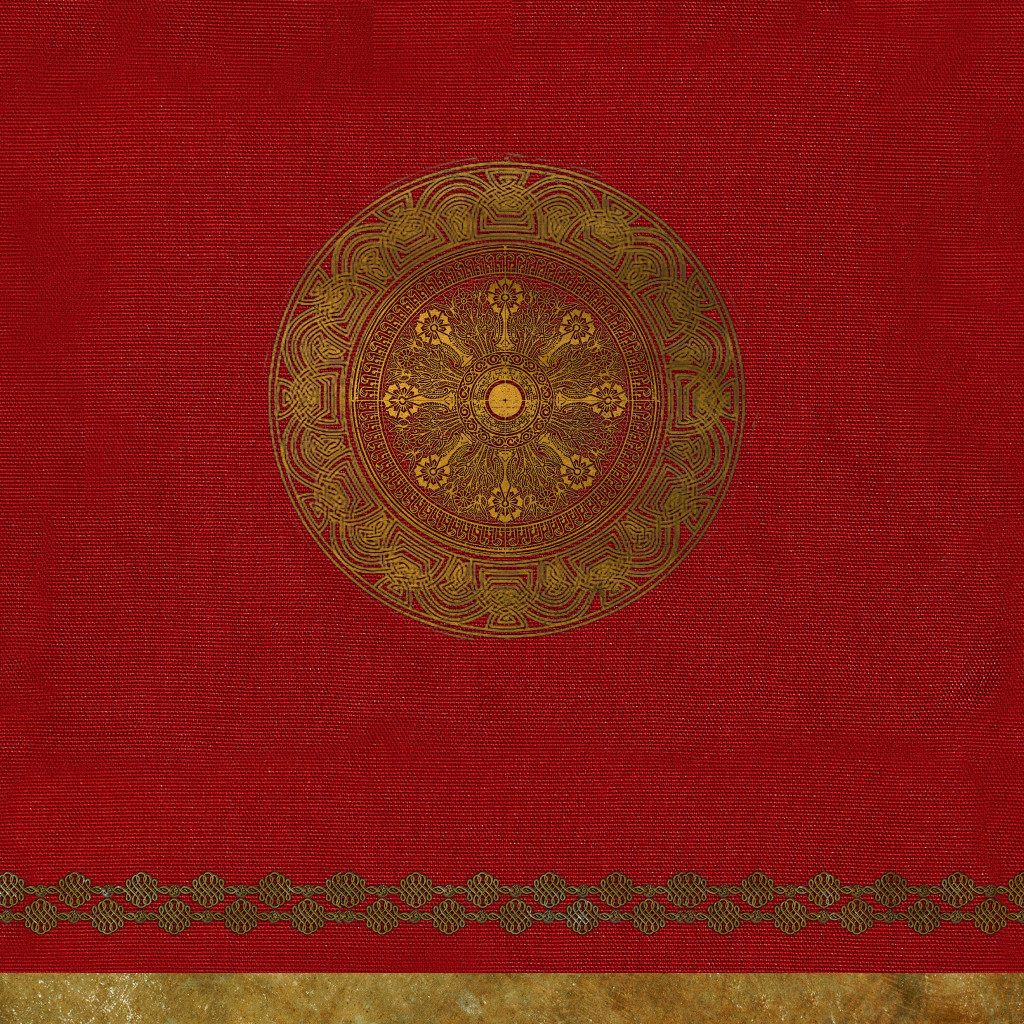
\includegraphics[width=\textwidth]{simluation/Sponza_Curtain_Red_diffuse.jpg}
\caption{Diffuser Reflexionsgrad}
\end{subfigure}
\begin{subfigure}[b]{0.24\textwidth}

\includegraphics[width=\textwidth]{simluation/Sponza_Curtain_Red_normal.jpg}
\caption{Oberflächennormale}
\end{subfigure}
\begin{subfigure}[b]{0.24\textwidth}
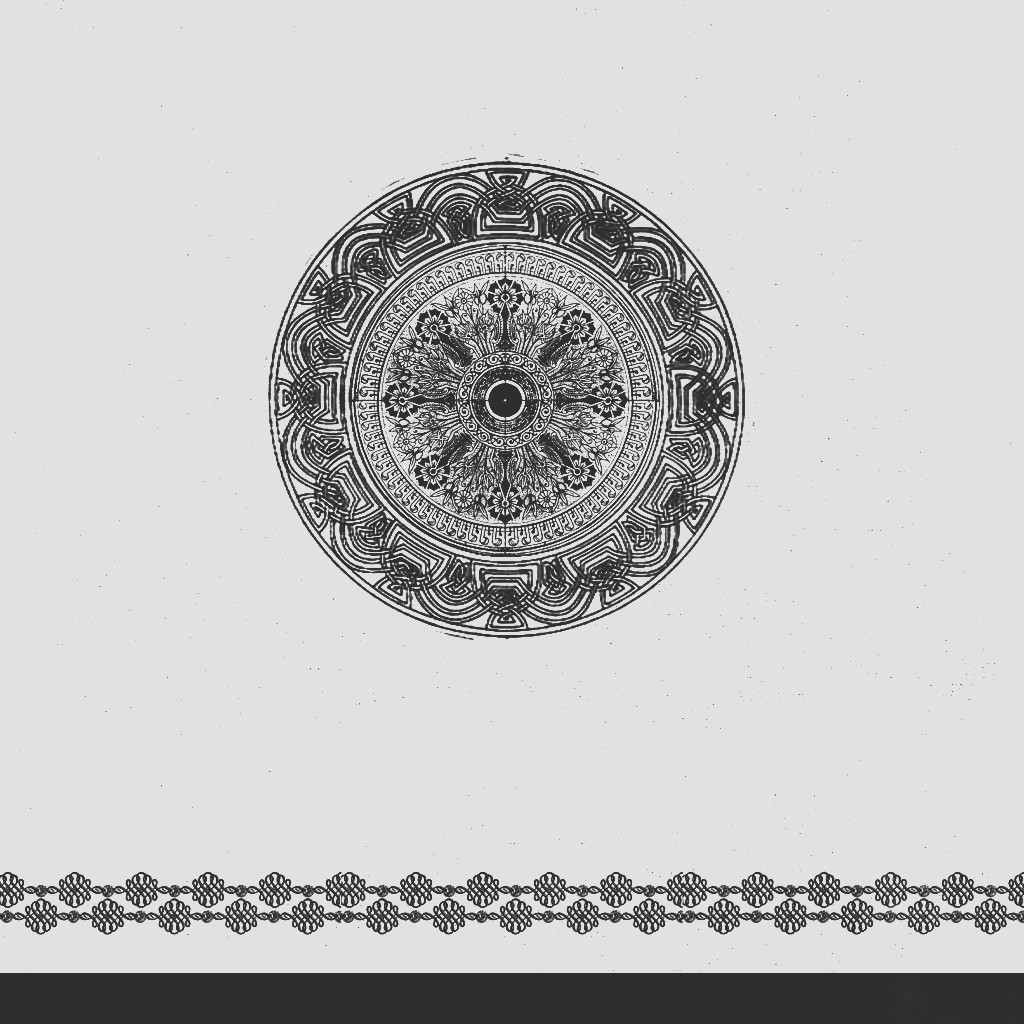
\includegraphics[width=\textwidth]{simluation/Sponza_Curtain_roughness.jpg}
\caption{Rauheit der Oberfläche}
\end{subfigure}
\begin{subfigure}[b]{0.24\textwidth}
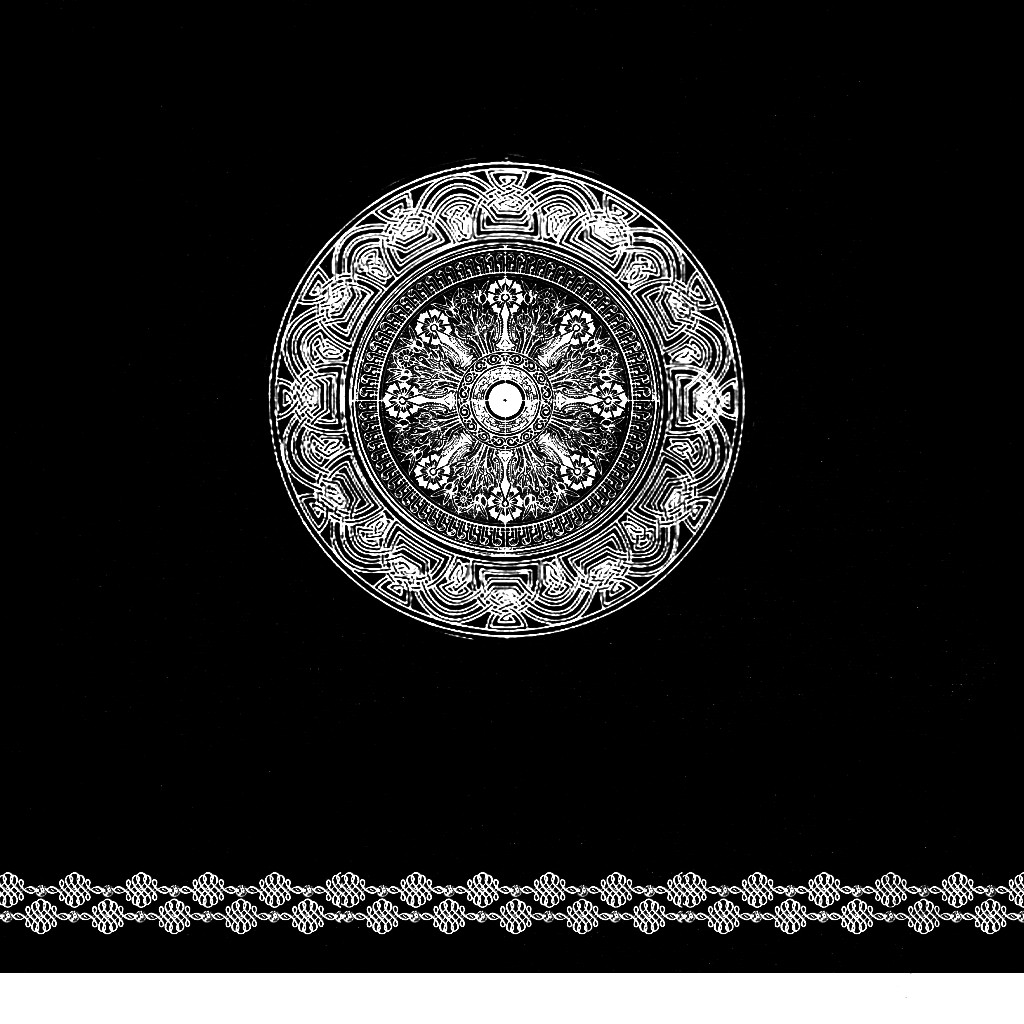
\includegraphics[width=\textwidth]{simluation/Sponza_Curtain_metallic.jpg}
\caption{Metallische Eigenschaften}
\end{subfigure}
\caption{Beispieltexturen einer verwendeten Testszene.}
\label{fig:material_textures}
\end{figure}

Das Closest Hit Programm wird ausgeführt, wenn der Strahl mit einer Oberfläche kollidiert. Dabei kann für jede Oberfläche ein eigenes Closest Hit Programm definiert werden. In dieser Arbeit wurde nur ein Programm für alle Oberflächen implementiert und die Materialeigenschaften werden als Texturen an die Grafikkarte übergeben. Diese Texturen enthalten dabei den diffusen Reflexionsgrad in Form einer 24 Bit RGB Farbe, die Rauheit der Oberfläche als 8 Bit Grauwert, die metallischen Eigenschaften als 8 Bit Maske und eine weitere Textur, die Details der Oberflächenstruktur in Form von Normalen der Oberfläche enthalten, die als 24 Bit RGB Farbe kodiert wurde. In \autoref{fig:material_textures} ist ein gewähltes Beispiel aus der Sponza Testszene zu sehen, die von Crytek erstellt wurde und häufig zum Testen von Lichtsimulationen verwendet wird.

Die Informationen, die in den Texturen übergeben werden, finden bei der Berechnung der BRDF Verwendung. Das Closest Hit Programm berechnet nach einer Kollision des Strahls mit der Oberfläche die Reflexionseigenschaften. Dazu wird wie in \autoref{sec:path_tracing} erläutert bei jedem Schnittpunkt ein neuer Strahl in zufälliger Richtung generiert und so für jedes Sample ein Pfad verfolgt. In dieser Arbeit wird zur Optimierung eine cosinusgewichtete Dichte der Strahlen verwendet, weshalb die Multiplikation mit $cos \theta_i$ aus der Rendergleichung entfällt. Der folgende Codeauszug veranschaulicht die Berechnung der indirekten Beleuchtung des Closest Hit Programms:
%
\begin{lstlisting}[escapeinside={(*}{*)}, numbers=right, language=C]
RT_PROGRAM void microfacet_closest_hit() {
    // Die gereiste Distanz des Strahls wird hier aufsummiert
    float3 hit_point = old_ray_origin + (ray_length * old_ray_direction);
    prd_radiance.ir_traveled_distance += length(old_ray_origin - hit_point);

    // Hier wird der Einfluss des direkten Lichts berechnet
    // Dieser unterscheidet sich je nach gewaehlter Modulation
    // ...
    
    // Der neue Strahl hat seinen Ursprung am Schnittpunkt
    prd_radiance.origin = hit_point;

    // Es wird eine neue Richtung fuer den Strahl berechnet
    prd_radiance.direction = cosine_sample_hemisphere(surface_normal); 
    
    // Der Abschwaechungfaktor der Reflextion wird bestimmt:
    // Es ist dabei bekannt, aus welcher Richtung der Strahl kommt und in welche
    // Richtung er reflektiert wird.

    // Es wird zwischen metallen und nicht-metallen unterschieden
    float3 fresnel;
    if(metallic) {
        // Hier wird der Fresnel Reflexionsgrad berechnet, falls die Oberflaeche metallisch ist
        fresnel = diffuse_reflectance * FrConductor(dot(prd_radiance.direction, half_vector), current_index_of_refraction, index_of_refraction, absorption_coefficien);
    } else {
        // Hier wird der Fresnel Reflexionsgrad berechnet, falls die Oberflaeche nicht metallisch ist
        fresnel = FrDielectric(dot(prd_radiance.direction, half_vector), current_index_of_refraction, index_of_refraction);
    }

    // Berechnung des diffusen Reflexionsanteils mittels Oren Nayar BRDF
    float3 diffuse = OrenNayar_f(diffuse_reflectance, surface_normal, -old_ray_direction, prd_radiance.direction, roughness) * (1.0f - fresnel) * (1.0f - metallic);
    
    // Berechnung des spiegelnden Reflexionsanteils mittels Torrance Sparrow BRDF
    float3 specular = TorranceSparrow_f(surface_normal, -old_ray_direction, prd_radiance.direction, fresnel, roughness);

    // Neue Berechnung des Abschwaechungsfaktors entsprechend des berechneten Reflexiongrades
    prd_radiance.attenuation = (diffuse + specular) * prd_radiance.attenuation * PI;
}
\end{lstlisting}
%
Auch hier handelt es sich um einen stark vereinfachten Auszug der Implementierung, der nur der Veranschaulichung dient. Dabei wurde die Berechnung der direkten Beleuchtung ausgeklammert, da diese sich für jede Art von Lichtquelle unterscheidet. Die Implementierung der direkten Beleuchtung wird daher in den folgenden Unterkapiteln jeweils im Detail erläutert.
%
\subsubsection{Pulsdauermodulation}

\begin{figure}[ht!]
\centering
\begin{subfigure}[b]{0.49\textwidth}
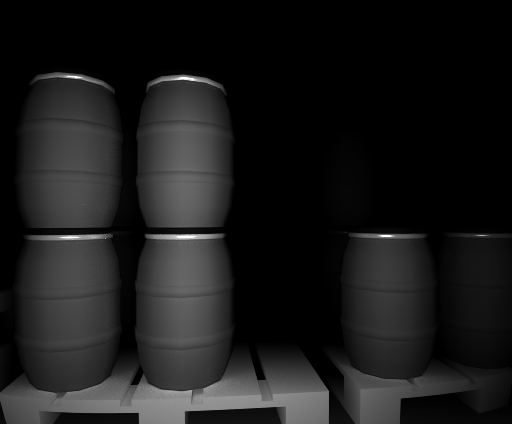
\includegraphics[width=\textwidth]{simluation/pulesd_phase_C1.png}
\caption{Intensität von $C_1$}
\end{subfigure}
\begin{subfigure}[b]{0.49\textwidth}
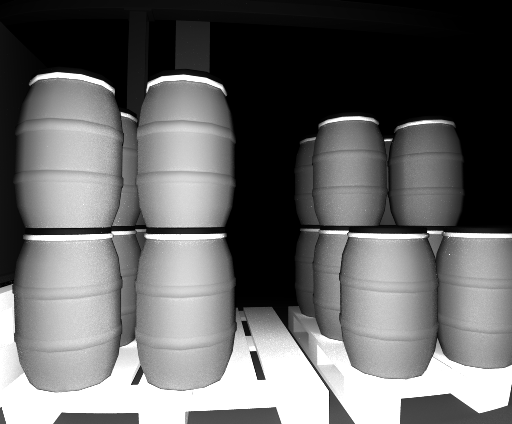
\includegraphics[width=\textwidth]{simluation/pulesd_phase_C2.png}
\caption{Intensität von $C_2$}
\end{subfigure}
\caption{Die Intensitäten der beiden Buckets $C_1$ und $C_2$, die bei der Simulation entstehen.}
\label{fig:pulsed_modulation_intensity}
\end{figure}

Im Folgenden wird die Berechnung der Intensitätsbilder für die Pulsdauermodulation erläutert. Bei der Pulsdauermodulation werden, wie in \autoref{chap:pulsed_tof} erläutert, zwei Intensitätsbilder erstellt, aus denen anschließend das Tiefenbild berechnet wird. \autoref{fig:pulsed_modulation_intensity} zeigt die beiden Intensitäten der Buckets $C_1$ und $C_2$, die in der Simulation berechnet werden. Dazu wird die Berechnung des Lichts des Path Tracing Algorithmus um den Faktor Zeit erweitert, die das Licht benötigt, um von einer Oberfläche reflektiert zu werden und beim Sensor aufzutreffen. Wie in \autoref{sec:closest_hit_program} ausgeführt, wird bei der Berechnung der indirekten Beleuchtung die Distanz, die das Licht gereist ist, aufsummiert. Bei jedem Schnittpunkt des Strahls mit der Oberfläche wird berechnet, ob dieser Punkt direkt beleuchtet wird. Dazu wird vom Schnittpunkt ein Strahl in die Richtung der Infrarot LEDs geschickt und getestet, ob sich auf dem direkten Weg zwischen der Oberfläche und der Lichtquelle ein Hindernis befindet. Falls die Lichtquelle vom Schnittpunkt aus sichtbar ist, wird die Oberfläche direkt durch das modulierte Licht der Infrarot LEDs beleuchtet. Zur Berechnung des reflektierten Anteils des Lichts in dem Zeitraum, in dem die Buckets geöffnet sind, wird zu der bis dahin zurückgelegten Strecke des Pfades die Distanz von der Lichtquelle zum Schnittpunkt hinzuaddiert, um die Gesamtstrecke zu erhalten, die das Licht zurückgelegt hat. Aus der Strecke und der Lichtgeschwindigkeit wird der Zeitversatz ermittelt, mit dem der Lichtpuls beim Sensor ankommt. Daraus lässt sich berechnen, welcher Teil des reflektierten Lichts im Bucket $C_1$ und welcher im Bucket $C_2$ gespeichert wird.

Der folgende Ausschnitt der Implementierung füllt die Lücke des vorangegangenen Codeauszugs:
%
\begin{lstlisting}[escapeinside={(*}{*)}, numbers=right, language=C]
// ...

// Berechnung der Pulslaenge anhand der genutzten Frequenz
const double pulselength = (1.0f / frequency) * 0.5f;

// Da das reflektierte Licht in zwei Buckets aufgeteilt wird, wird hier ein 2D Vektor zum Speichern verwendet
float2 ir_result_pulse = make_float2(0.0f);

unsigned int num_ir_lights = ir_lights.size();
for(int i = 0; i < num_ir_lights; ++i) {
    // Berechnung einiger nuetlicher Variablen
    BasicLight light = ir_lights[i];
    float3 light_direction = light.pos - hit_point;
    float light_distance = sqrt(dot(light_direction, light_direction));
    light_direction = light_direction / light_distance;

    float NdotL = saturate(dot(surface_normal, light_direction));
    if (NdotL > 0.0f) {

        // Berechne einen Strahl vom Schnittpunkt zur Lichtquelle um zu bestimmen, ob sich die Oberflaeche im Schatten befindet oder direkt beleuchtet wird
        PerRayData_shadow shadow_prd;
        Ray shadow_ray = make_Ray( hit_point, light_direction, shadow_ray_type, scene_epsilon, light_distance - scene_epsilon );
        rtTrace(top_object, shadow_ray, shadow_prd);

        if(!shadow_prd.inShadow) {

            // Hier wird genau wie bereits beschrieben der diffuse und spekulare Anteil der Reflexion berechnet
            // ...
            
            float Intensity = prd_radiance.ir_attenuation * luminanceCIE((diffuse + specular) * (light.color * light.intensity * (NdotL / dot(light_direction, light_direction))));

            // Berechne anhand der gereisten Distanz den Zeitversatz, an dem die Strahlung wieder beim Sensor auftrifft 
            float sourceToSensorDistance = light_distance + prd_radiance.ir_traveledDistance;
            float deltaTime = sourceToSensorDistance / speedOfLight;

            // Bestimme den Startzeitpunkt, an denen die Buckets beginnen Licht aufzunehmen
            float C1_start = 0.0f;
            float C2_start = pulselength;
            
            // Bestimme den Anfangszeitpunkt und den Endzeitpunkt des reflektierten Lichtpulses
            float begin = deltaTime;
            float end = deltaTime + pulselength;

            // Bestimme den Anteil der Ladung, der von C1 aufgenommen wird
            if((end >= C1_start && end <= C1_start + pulselength) || (begin >= C1_start && begin <= C1_start + pulselength)) {
                if(begin > C1_start)
                    ir_result_pulse.x += (((C1_start + pulselength) - begin) / pulselength) * Intensity;
                else
                    ir_result_pulse.x += ((end - C1_start) / pulselength) * Intensity;
            }
            
            // Bestimme den Anteil der Ladung, der von C2 aufgenommen wird
            if((end >= C2_start && end <= C2_start + pulselength) || (begin >= C2_start && begin <= C2_start + pulselength)) {
                if(begin > C2_start)
                    ir_result_pulse.y += (((C2_start + pulselength) - begin) / pulselength) * Intensity;
                else
                    ir_result_pulse.y += ((end - C2_start) / pulselength) * Intensity;
            }
        }
    }
}

// Gebe das Ergebnis an das Ray Generation Programm zurueck
prd_radiance.radiance = ir_result_pulse;

// ...
\end{lstlisting}
%
\subsubsection{Rechteckförmige Wellenfunktion}\label{sec:simulation_rectangle_tof}

\begin{figure}[ht!]
\centering
\begin{subfigure}[b]{0.24\textwidth}
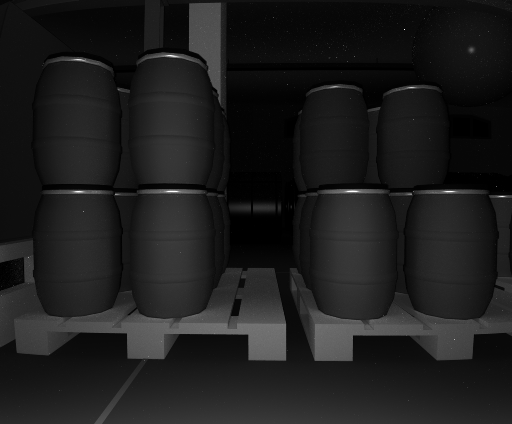
\includegraphics[width=\textwidth]{simluation/cw_phase_C1.png}
\caption{Intensität $C_1$}
\end{subfigure}
\begin{subfigure}[b]{0.24\textwidth}
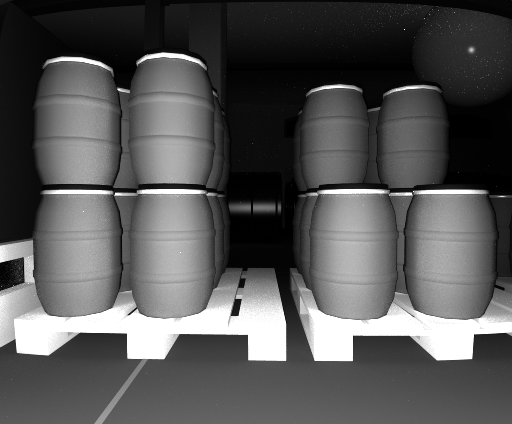
\includegraphics[width=\textwidth]{simluation/cw_phase_C2.png}
\caption{Intensität $C_2$}
\end{subfigure}
\begin{subfigure}[b]{0.24\textwidth}
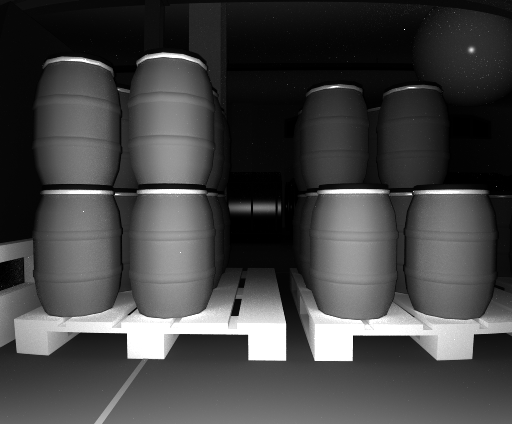
\includegraphics[width=\textwidth]{simluation/cw_phase_C3.png}
\caption{Intensität $C_3$}
\end{subfigure}
\begin{subfigure}[b]{0.24\textwidth}
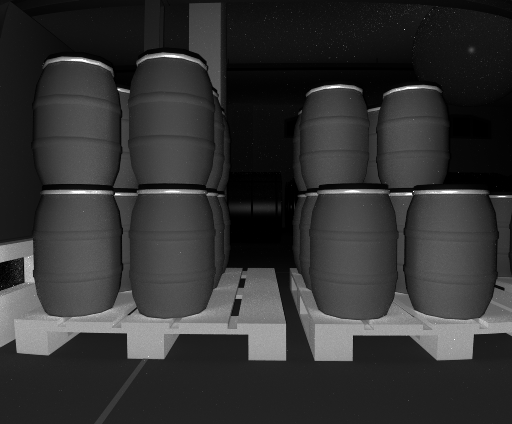
\includegraphics[width=\textwidth]{simluation/cw_phase_C4.png}
\caption{Intensität $C_4$}
\end{subfigure}
\caption{Die Intensitäten der Buckets $C_1$, $C_2$, $C_3$ und $C_4$, die bei der Simulation der Continuous-Wave Modulation entstehen.}
\label{fig:cw_modulation_intensity}
\end{figure}

Die Simulation der Phasenbilder für die Continuous-Wave Modulation verläuft ähnlich zur Implementierung der Pulsdauermodulation. Die Continuous-Wave Modulation unterscheidet sich von der Pulsdauermodulation in zwei Aspekten:

\begin{enumerate}
    \item Es werden, wie in \autoref{chap:cw_tof} erläutert, vier statt zwei Buckets verwendet, um das reflektierte Licht aufzunehmen.
    \item Statt eines Pulses wird eine Welle emittiert, wobei die rechteckförmige Wellenfunktion als eine sich periodisch wiederholende, Pulsdauermodulation betrachtet werden kann.
\end{enumerate}

Die Ähnlichkeit der rechteckförmigen Wellenfunktion zur Pulsdauermodulation wird genutzt und die Ladung der Buckets wird auf dieselbe Weise simuliert. Dazu wird die Berechnung zunächst um zwei zusätzliche Buckets erweitert und das Zeitfenster, in dem die Buckets offen sind, wie zuvor berechnet. Da im Gegensatz zur Pulsdauermodulation eine periodische Welle emittiert wird, müssen alle vorherigen Lichtpulse der Berechnung berücksicht werden. Dazu wird der Lichtpuls so lange um seine doppelte Pulslänge verschoben und die Verteilung auf die vier Buckets für jeden Lichtpuls berechnet, bis die komplette Welle bei der Berechnung der Ladung der Buckets berücksichtigt worden ist.

Der folgende Auszug aus der Implementierung veranschaulicht die Berechnung der Phasenbilder für die Continuous-Wave Modulation von rechteckförmigen Wellenfunktionen:
\begin{lstlisting}[escapeinside={(*}{*)}, numbers=right, language=C]
// ...

// Da das reflektierte Licht in vier Buckets aufgeteilt wird, wird hier ein 4D Vektor zum Speichern verwendet
float4 ir_result_rect = make_float4(0.0f);

// ...

// Berechne den Zeitraum, in denen die Buckets offen sind und Licht aufnehmen
float C1_start = 0.0f;
float C2_start = pulselength;
float C3_start = pulselength * 0.5f;
float C4_start = (pulselength * 0.5f) + pulselength;

// Verschiebe den Lichtpuls so lange in die Vergangenheit, bis er ausserhalb des Messrahmens der vier Buckets liegt
while(deltaTime < C4_start + pulselength) {
    deltaTime = deltaTime + (pulselength * 2.0);
}

// Berechne die Intensitaetsverteilung analog zur Pulsdauermodulation fuer jeden einzelnen Lichtpuls
while(deltaTime + pulselength > 0.0f) {
    float begin = deltaTime;
    float end = deltaTime + pulselength;

    if((end >= C1_start && end <= C1_start + pulselength) || (begin >= C1_start && begin <= C1_start + pulselength)) {
        if(begin > C1_start)
            ir_result_rect.x += (((C1_start + pulselength) - begin) / pulselength) * Intensity;
        else
            ir_result_rect.x += ((end - C1_start) / pulselength) * Intensity;
    }
    
    if((end >= C2_start && end <= C2_start + pulselength) || (begin >= C2_start && begin <= C2_start + pulselength)) {
        if(begin > C2_start)
            ir_result_rect.y += (((C2_start + pulselength) - begin) / pulselength) * Intensity;
        else
            ir_result_rect.y += ((end - C2_start) / pulselength) * Intensity;
    }

    if((end >= C3_start && end <= C3_start + pulselength) || (begin >= C3_start && begin <= C3_start + pulselength)) {
        if(begin > C3_start)
            ir_result_rect.z += (((C3_start + pulselength) - begin) / pulselength) * Intensity;
        else
            ir_result_rect.z += ((end - C3_start) / pulselength) * Intensity;
    }
    
    if((end >= C4_start && end <= C4_start + pulselength) || (begin >= C4_start && begin <= C4_start + pulselength)) {
        if(begin > C4_start)
            ir_result_rect.w += (((C4_start + pulselength) - begin) / pulselength) * Intensity;
        else
            ir_result_rect.w += ((end - C4_start) / pulselength) * Intensity;
    }

    // Verschiebe den Lichtpuls um seine doppelte Phasenlaenge um den zeitlich folgenden Lichtpuls zu berechnen
    deltaTime = deltaTime - (pulselength * 2.0);
}

// ...
\end{lstlisting}
%
Die aus der Simulation resultierenden Ladungen der einzelnen Buckets werden in Form von Phasenbildern in \autoref{fig:cw_modulation_intensity} veranschaulicht.
%
\subsubsection{Sinusförmige Wellenfunktion}
%
Bei der sinusförmigen Wellenfunktion handelt es sich um die simpelste Berechnung zur Phasenverschiebung. Dazu wird für jeden Bucket der Flächeninhalt unter der Wellenfunktion für den Abschnitt berechnet, in denm die Buckets offen sind:
\begin{equation}Q_{k}=\frac{\alpha \cdot \Big(\cos(2 \pi f \cdot t_{start}) - \cos(2 \pi f \cdot t_{end}) \Big)}{2 \pi f} - (\beta \cdot t_{start}) + (\beta \cdot t_{end}).\end{equation}

Dabei ist $\alpha$ die Amplitude der Funktion, $f$ die Frequenz, $\beta$ der Versatz, $k$ der Index des Buckets und $t_{start}$ und $t_{start}$ die End- und Startzeit, in der ein Bucket geöffnet ist.

Folgender Codeauszug zeigt abschließend die Berechnung der Phasenbilder für die sinusförmige Wellenfunktion:
%
\begin{lstlisting}[escapeinside={(*}{*)}, numbers=right, language=C]
// ...

// Da das reflektierte Licht in vier Buckets aufgeteilt wird, wird hier ein 4D Vektor zum Speichern verwendet
float4 ir_result_sin = make_float4(0.0f);

// ...

ir_result_sin.x += Intensity * getArea(frequency, C1_start - deltaTime, (C1_start - deltaTime) + pulselength);
ir_result_sin.y += Intensity * getArea(frequency, C2_start - deltaTime, (C2_start - deltaTime) + pulselength);
ir_result_sin.z += Intensity * getArea(frequency, C3_start - deltaTime, (C3_start - deltaTime) + pulselength);
ir_result_sin.w += Intensity * getArea(frequency, C4_start - deltaTime, (C4_start - deltaTime) + pulselength);

// ...

\end{lstlisting}
%
Die Phasenbilder unterscheiden sich nur minimal von denen der rechteckförmigen Wellenfunktion, die in \autoref{fig:cw_modulation_intensity} zu sehen sind.
%
\subsection{Miss Programm}

\begin{figure}[ht!]
\centering
\begin{subfigure}[b]{0.49\textwidth}
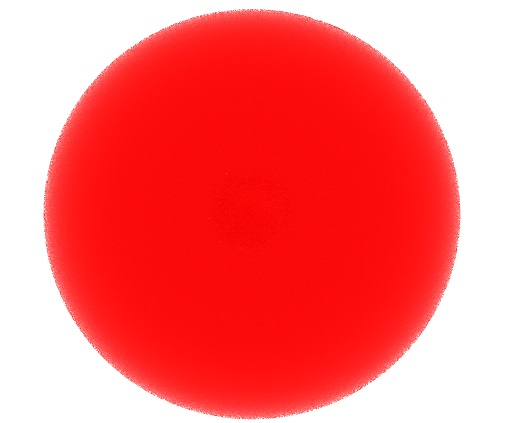
\includegraphics[width=\textwidth]{simluation/Red_Sphere_White_Background.jpg}
\caption{Rote Plastiksphäre bei konstanter Hintergrundbeleuchutng}
\label{fig:miss_programm_const_background}
\end{subfigure}
\begin{subfigure}[b]{0.49\textwidth}
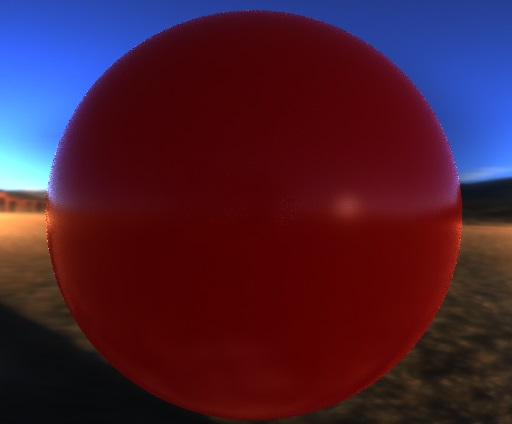
\includegraphics[width=\textwidth]{simluation/Red_Sphere_envmap_Background.jpg}
\caption{Rote Plastiksphäre bei einer Beleuchtung durch eine Environment Map}
\label{fig:miss_programm_environment_map}
\end{subfigure}
\caption{Mit einem Miss Programm können sowohl eine konstante Hintergrundbeleuchtung als auch eine eingemessene Beleuchtung durch eine Environment Map genutzt werden.}
\label{fig:miss_programm}
\end{figure}

Das Miss Programm wird aufgerufen, sobald der Strahl die Szene verlässt und keine Kollision mit der Geometrie mehr stattfinden kann. Dabei kann der Pfad einfach beendet werden oder für den Hintergrund eine Strahlung festgelegt werden, was zu einer Umgebungsbeleuchtung führt. Die Simulation des Umgebungslichts wirkt sich auf den zufälligen Fehler der Tiefenwerte aus, weshalb diese in dieser Arbeit relevant ist.

Folgender Codeauszug veranschaulicht die Verwendung eines konstanten Hintergrundes als Strahlungsquelle:
\begin{lstlisting}[escapeinside={(*}{*)}, numbers=right, language=C]
RT_PROGRAM void miss()
{
    prd_radiance.radiance = prd_radiance.attenuation * background_color;
    prd_radiance.done = true;
}
\end{lstlisting}
%
Falls für den Hintergrund ein Wert größer als Null gewählt wird, wird die Umgebung als Strahlungsquelle betrachtet, falls der Strahl die Szene verlässt (siehe \autoref{fig:miss_programm_const_background}). Alternativ lässt sich hier eine eingemessene Umgebungsbeleuchtung nutzen, die als Strahlungsquelle dient, falls der Strahl die Szene verlässt (siehe \autoref{fig:miss_programm_environment_map}). Dazu wird eine sogenannte \emph{Environment Map} aufgenommen und auf eine Sphäre projiziert, die die Kamera umgibt. Falls der Strahl die Szene verlässt, wird die Schnittstelle mit der Sphäre berechnet und die Strahlung aus der entsprechenden Richtung bestimmt.

Folgender Codeauszug veranschaulicht die Verwendung einer Environment Map als Strahlungsquelle:
\begin{lstlisting}[escapeinside={(*}{*)}, numbers=right, language=C]
rtTextureSampler<float4, 2> envmap;
RT_PROGRAM void envmap_miss()
{
    float theta = atan2f( ray.direction.x, ray.direction.z );
    float phi   = M_PIf * 0.5f -  acosf( ray.direction.y );
    float u     = (theta + M_PIf) * (0.5f * M_1_PIf);
    float v     = 0.5f * ( 1.0f + sinf(phi) );

    prd_radiance.radiance = prd_radiance.attenuation * make_float3( tex2D(envmap, u, v) );
    prd_radiance.done = true;
}
\end{lstlisting}
%
\section{Tiefenbildgenerierung aus den Phasenbildern}\label{sec:depth_by_phase}
%
m folgenden Abschnitt wird darauf eingegangen, wie aus den einzelnen Phasenbildern Tiefenbilder errechnet werden. Die Simulation der Lichtausbreitung mittels Path Tracing liefert je nach gewählter Modulation und Anzahl der verwendeten Buckets zwei oder vier Phasenbilder, aus denen die Tiefeninformationen berechnet werden. Dazu wird, wie in \autoref{chap:time_of_flight} erläutert, vorgegangen und die Distanz wird entweder direkt aus dem Verhältnis der zwei Buckets berechnet oder über die Phasenverschiebung ermittelt. Bei den Tiefeninformationen handelt es sich um eine radiale Distanz von der Blende der Kamera zum Objekt. Bei der radialen Distanz handelt es sich um die Länge eines Vektors, dessen Ursprung mit dem des Kamerakoordinatensystems übereinstimmt. Da für jeden Pixel für den Path Tracing Algorithmus Strahlen berechnet wurden, ist bereits bekannt, in welche Richtung der Vektor zeigt, aus dem die Tiefeninformation ermittelt wurde. Um aus den Tiefeninformationen eine 3D Koordinate zu berechnen, wird der Vektor um die ermittelte radiale Distanz verlängert, die bei der Berechnung der Phase ermittelt wurde. 

Time-of-Flight Kamerasysteme liefern häufig anstelle einer radialen Distanz eine Tiefe als Ergebnis. Dazu wird zunächst die 3D Koordinate im Raum berechnet und ausschließlich der Z-Wert der Koordinate in einem Tiefenbild an den Nutzer übergeben, worauf hier allerdings verzichtet wird, weshalb im Folgenden von Distanzbildern gesprochen wird.

Wie in \autoref{chap:analysis} erläutert, sind die Distanzen äußeren Einflüssen unterworfen, was zu Fehlern im Distanzbild führt. Die Simulation dieser Fehler wird im Folgenden erläutert. 
%
\subsection{Simulation des Lens Scattering und des Mixed Pixels Fehlers}
%
Bei der genaueren Untersuchung des Mixed Pixels Fehler in \autoref{sec:mixed_pixels} wurde die Vermutung angestellt, dass sich dieser auf den Lens Scattering Effekt zurückführen lässt, weshalb nur der Lens Scattering Fehler simuliert wird und der Mixed Pixels Fehler dadurch ebenfalls berücksichtigt wird. Bei der genauen Untersuchung des Einflusses heller Pixel auf die benachbarten Pixel in \autoref{sec:lens_scattering} wurde eine Punktspreizfunktion ermittelt, mit der sich dieser Effekt nachbilden lässt. Dazu wird aus der Funktion eine \emph{Faltungsmatrix} definiert, die auf jedes Phasenbild angewandt wird. Das führt dazu, dass sich die Intensitäten auf die Nachbarpixel verteilen, wordurch die Fehler im Tiefenbild verursacht werden. Die Ergebnisse der Simulation werden in \autoref{chap:evaluation} ausführlich Detail besprochen.
%
\subsection{Simulation des zufälligen Fehlers}
%
Der zufällige Fehler wird nach der \autoref{eq:timeofflighterror} implementiert. Dazu werden die Intensität $A$ des Infrarotsignals und der Versatz $B$ aus den Phasenbildern berechnet. In den Versatz $B$ fließt zusätzlich das Umgebungslicht ein, das durch das Miss Programm simuliert wird, während die Intensität $A$ ausschließlich die modulierte Strahlung der Infrarot LEDs enthält, selbst wenn das Umgebungslicht einen Einfluss auf die einzelnen Intensitätsbilder ausübt. Die Pulsdauermodulation ist davon allerdings ausgeschlossen, da sich hier das Umgebungslicht nicht aus den Phasenbildern herausrechnen lässt.

Der zufällige Fehler wird dabei zum resultierenden Distanzbild addiert. Dazu wird die Implementierung der Normalverteilung der Standard Template Library verwendet. Diese erwartet die Standardabweichung $\sigma$ als Parameter, der in der \autoref{eq:timeofflighterror} berechnet wurde. 

Der folgende Codeauszug demonstriert die Berechnung der modifizierten Distanz mittels einer Normalverteilung:
%
\begin{lstlisting}[escapeinside={(*}{*)}, numbers=right, language=C++]
// ...

// Definition eines Zufallsgenerators
std::default_random_engine g_generator;

// ...

float distance = (speedOfLight / (4.0f * M_PIf * frequency)) * phi;
if (distance != 0.0f && m_noise_enabled)
{
    // Berechnung des Rauschens mittels der Normalverteilung
    std::normal_distribution<double> distribution(distance, standard_deviation);
    double imperfectDistance = distribution(g_generator);

    // Umrechnung von Meter auf Millimeter
    output_depth[launch_index] = imperfectDistance * 1000.0f;
}

// ...
\end{lstlisting}

\subfilebib % Makes bibliography available when compiling as subfile
\end{document}
